\documentclass[runningheads]{llncs}
\usepackage[T1]{fontenc}
\usepackage{graphicx}
\usepackage{booktabs}
\usepackage{multirow}
\usepackage{amsmath}
\usepackage{url}
\usepackage[hidelinks]{hyperref}
\usepackage[section]{placeins}
\graphicspath{{figures/}}
\pagestyle{plain}
\raggedbottom
\setlength{\textfloatsep}{6pt plus 1pt minus 2pt}
\setlength{\floatsep}{6pt plus 1pt minus 2pt}
\setlength{\intextsep}{6pt plus 1pt minus 2pt}
\setlength{\abovecaptionskip}{5pt}
\setlength{\belowcaptionskip}{2pt}
\renewcommand{\topfraction}{0.9}
\renewcommand{\textfraction}{0.08}
\renewcommand{\floatpagefraction}{0.8}
\begin{document}

\title{PlasmaXAI: Counterfactual-Guided Explainable Fusion for Malignant Plasma Cell Recognition and Patient-Level Morphologic Consistency Analysis}
\titlerunning{PlasmaXAI}
\author{Arnob Aich Anurag}
\institute{American International University-Bangladesh, Dhaka, Bangladesh}
\authorrunning{Anurag et al.}

\maketitle
\thispagestyle{plain}

\begin{abstract}
Accurate plasma cell recognition is essential for multiple myeloma screening, yet routine microscopic assessment remains labor-intensive, subjective, and difficult to scale in resource-constrained settings. This paper presents PlasmaXAI, an explainable computational pathology framework that combines frozen ResNet50 and DenseNet121 image embeddings with handcrafted morphology, a morphology-derived counterfactual boundary model, and learned fusion gates that inject counterfactual information directly into the classification pathway. Evaluated on PCMMD, PlasmaXAI achieves 93.42\% accuracy, 93.43\% weighted F1, 91.24\% plasma precision, 94.63\% plasma recall, and 97.76\% AUC at the selected precision-recall balanced operating point. Beyond standard classification, the framework provides counterfactual explanation analysis, calibration and bootstrap summaries, ablation evidence, and exploratory patient-level robustness results. PlasmaXAI is therefore positioned as an interpretable screening framework rather than a black-box classifier, with practical relevance for digital hematopathology workflows that need both strong discrimination and transparent reasoning.
\keywords{Multiple myeloma \and Digital pathology \and Explainable AI \and Counterfactual analysis \and Plasma cell recognition \and Deep learning}
\end{abstract}

\section{Introduction}
Multiple myeloma is a plasma-cell malignancy in which microscopic morphology remains central to diagnosis, risk assessment, and disease monitoring \cite{mmreview}. In routine practice, stained marrow smears are reviewed manually, a process that is time-consuming and vulnerable to inter-observer variability, stain heterogeneity, and heavy workload. These limitations become more pronounced in laboratories where specialist review time is limited and digital pathology support is still developing.

Deep learning has already transformed medical image analysis and digital pathology, but strong classification accuracy alone is not enough for clinical adoption \cite{litjens,bera,campanella}. A model used for plasma cell assessment should not only identify malignant likelihood, but also expose the evidence that drives its decision so that users can calibrate, audit, and question the output when needed.

PlasmaXAI is designed with that objective. Instead of treating explainability as a post-hoc add-on, it incorporates counterfactual morphology signals directly into a learned fusion model. The resulting framework combines deep image representation, handcrafted cell morphology, counterfactual distance-to-boundary reasoning, and modality gating in one decision path. This paper contributes three main elements: an explainable multi-branch classifier for malignant plasma cell recognition, a counterfactual-aware fusion strategy, and an evaluation protocol that extends beyond accuracy to calibration, ablation, and patient-level robustness.

\section{Literature Review}
Modern digital pathology systems rely heavily on convolutional neural networks because they learn hierarchical cell and tissue representations more effectively than handcrafted descriptors alone \cite{litjens,janowczyk}. In practice, clinically useful models must balance local texture sensitivity with stable higher-level semantics \cite{bera,campanella}. Residual networks improve optimization through identity mappings, whereas densely connected networks encourage feature reuse and strong gradient flow \cite{resnet,densenet}. Encoder-decoder families such as U-Net and attention-augmented U-Net further demonstrate that carefully designed feature fusion can improve biomedical visual reasoning \cite{unet,attentionunet}. These families are relevant to plasma cell analysis because malignant recognition depends on both fine-grained chromatic cues and broader morphologic structure.

Explainability research has developed along several complementary directions, including local surrogate explanations, saliency-based visualization, feature-attribution methods, and counterfactual reasoning \cite{lime,gradcam,shap,wachter}. Among these, counterfactual explanations are especially attractive in healthcare because they express model behavior through clinically intuitive change statements: what minimal feature shift would move a prediction toward a different outcome? Wachter et al. formalized this idea for automated decision systems \cite{wachter}, while DICE showed how diverse counterfactual sets can improve interpretation quality \cite{diceml}. Calibration is equally important, because a high-confidence prediction is clinically useful only when predicted probability aligns with observed frequency \cite{calibration}. PlasmaXAI builds on these strands by treating counterfactual information as a model input as well as an explanatory output.

\section{Materials and Methods}
\subsection{Dataset and Feature Construction}
The experiments use PCMMD cell images arranged into a cell-level training corpus and a separate patient-organized cohort for exploratory patient analysis. Each image is resized to 224 $\times$ 224 and normalized for CNN feature extraction. In parallel, a morphology pipeline computes nucleus-to-cytoplasm ratio, nucleus area, cytoplasm area, staining intensity, granularity, roundness, and mean RGB channels. These descriptors form an interpretable phenotype layer that complements the learned image features.

\subsection{PlasmaXAI Architecture}
PlasmaXAI combines two frozen image backbones, ResNet50 and DenseNet121, with morphology, counterfactual, and score branches. A logistic morphology model first estimates a counterfactual decision boundary in handcrafted feature space. From that boundary, the system derives feature-shift and distance terms that quantify how a sample would need to change in order to move toward the benign region.

The fusion model processes ResNet, DenseNet, morphology, counterfactual, and score streams through separate encoders. Counterfactual signals modulate the image features through sigmoid gates, refine the score branch, and contribute to a softmax modality gate that controls final fusion weights. This makes the counterfactual path structurally relevant rather than merely descriptive. Figure~\ref{fig:arch} presents the high-level workflow and the detailed internal architecture.

\begin{figure}[!htbp]
\centering
\begin{minipage}[t]{0.48\textwidth}
\centering
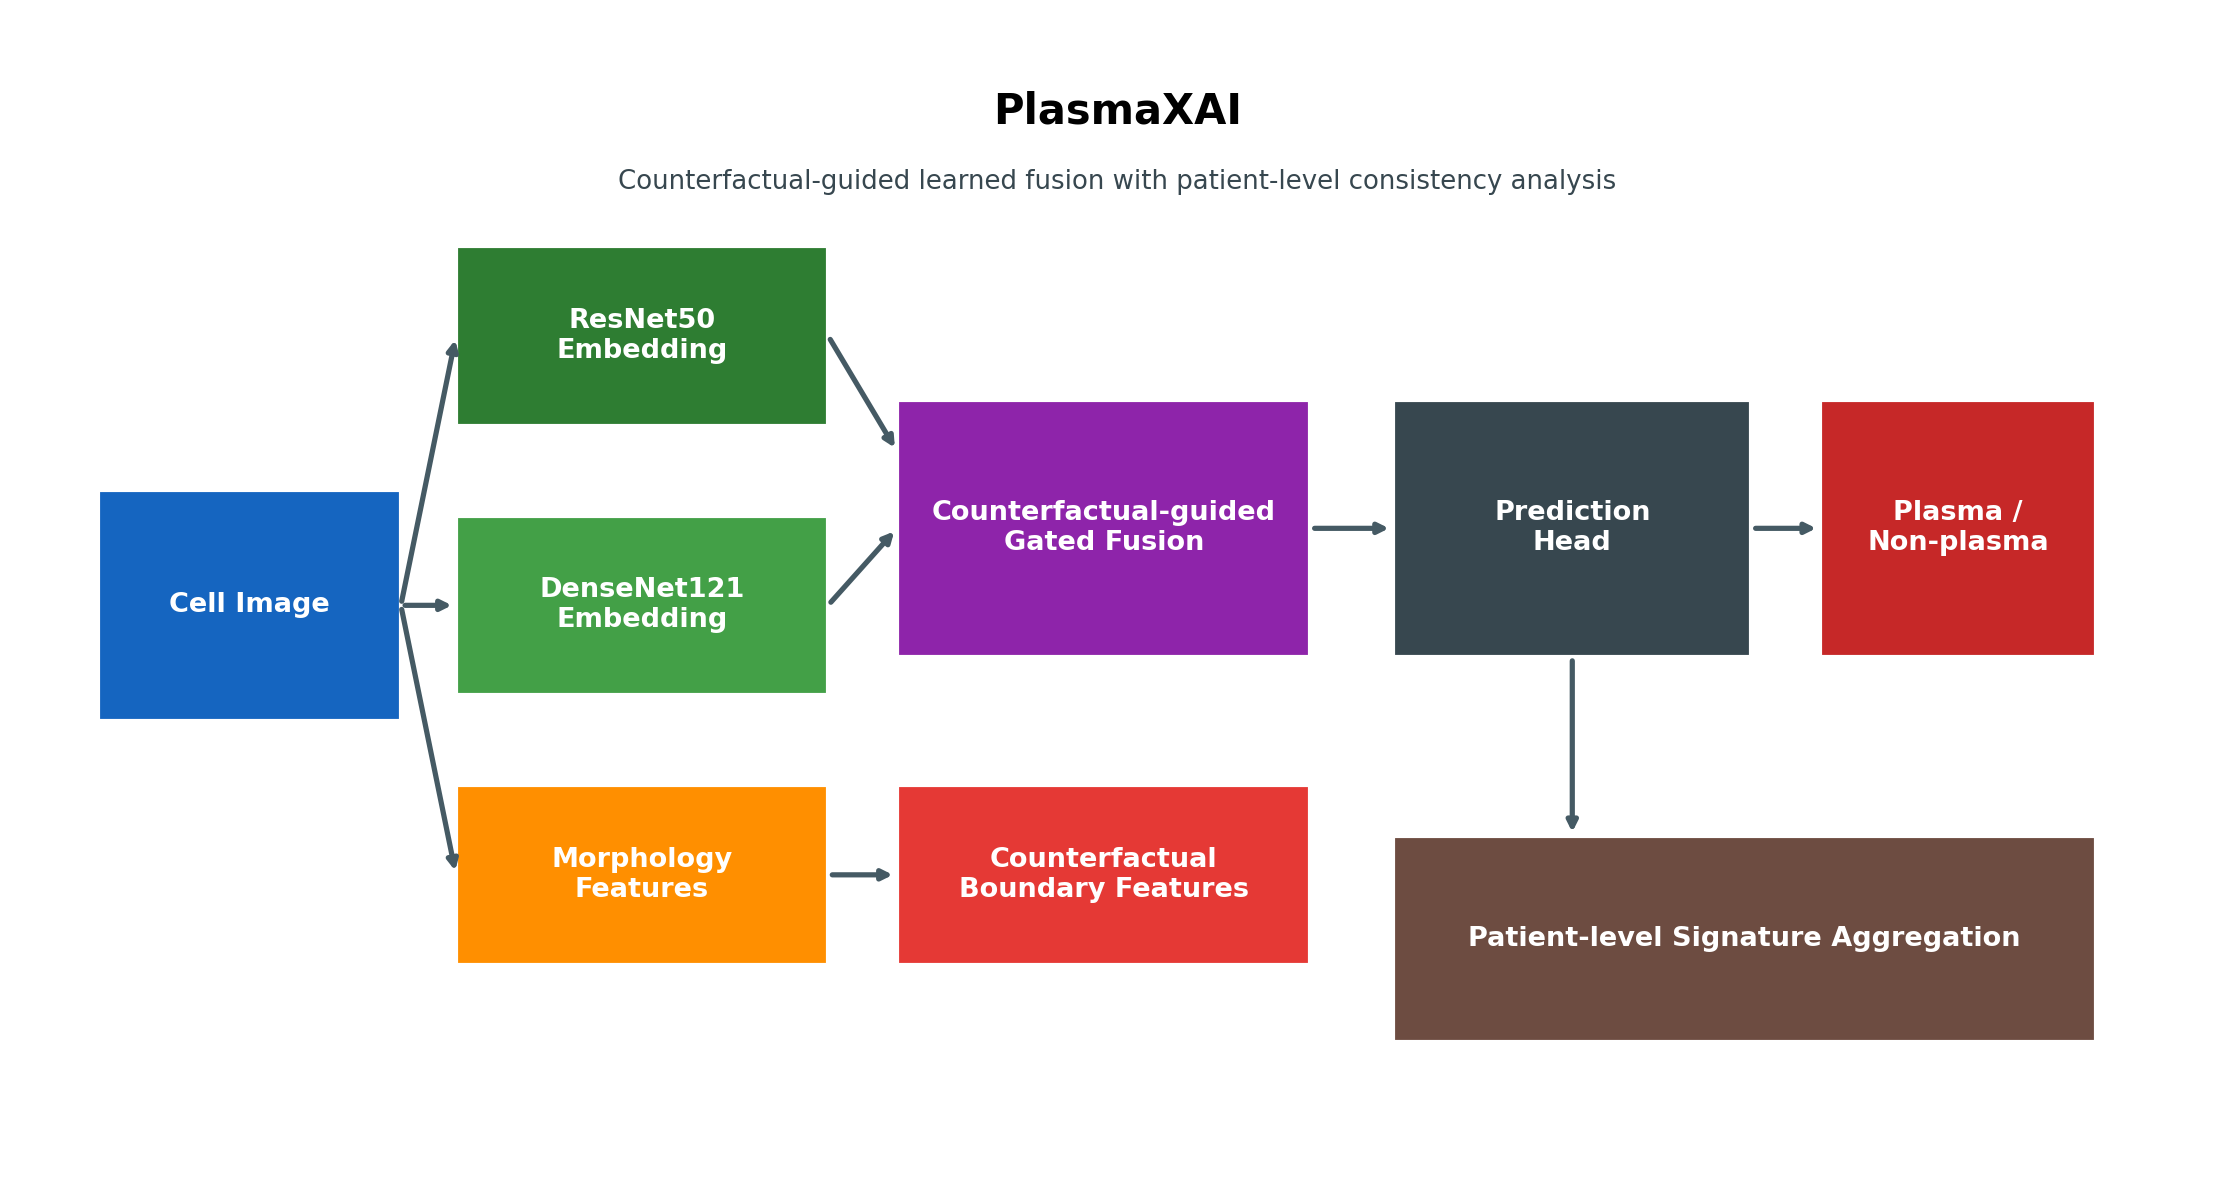
\includegraphics[width=\linewidth]{plasmaxai_framework.png}\\[2pt]
\small (a) High-level PlasmaXAI workflow.
\end{minipage}\hfill
\begin{minipage}[t]{0.48\textwidth}
\centering
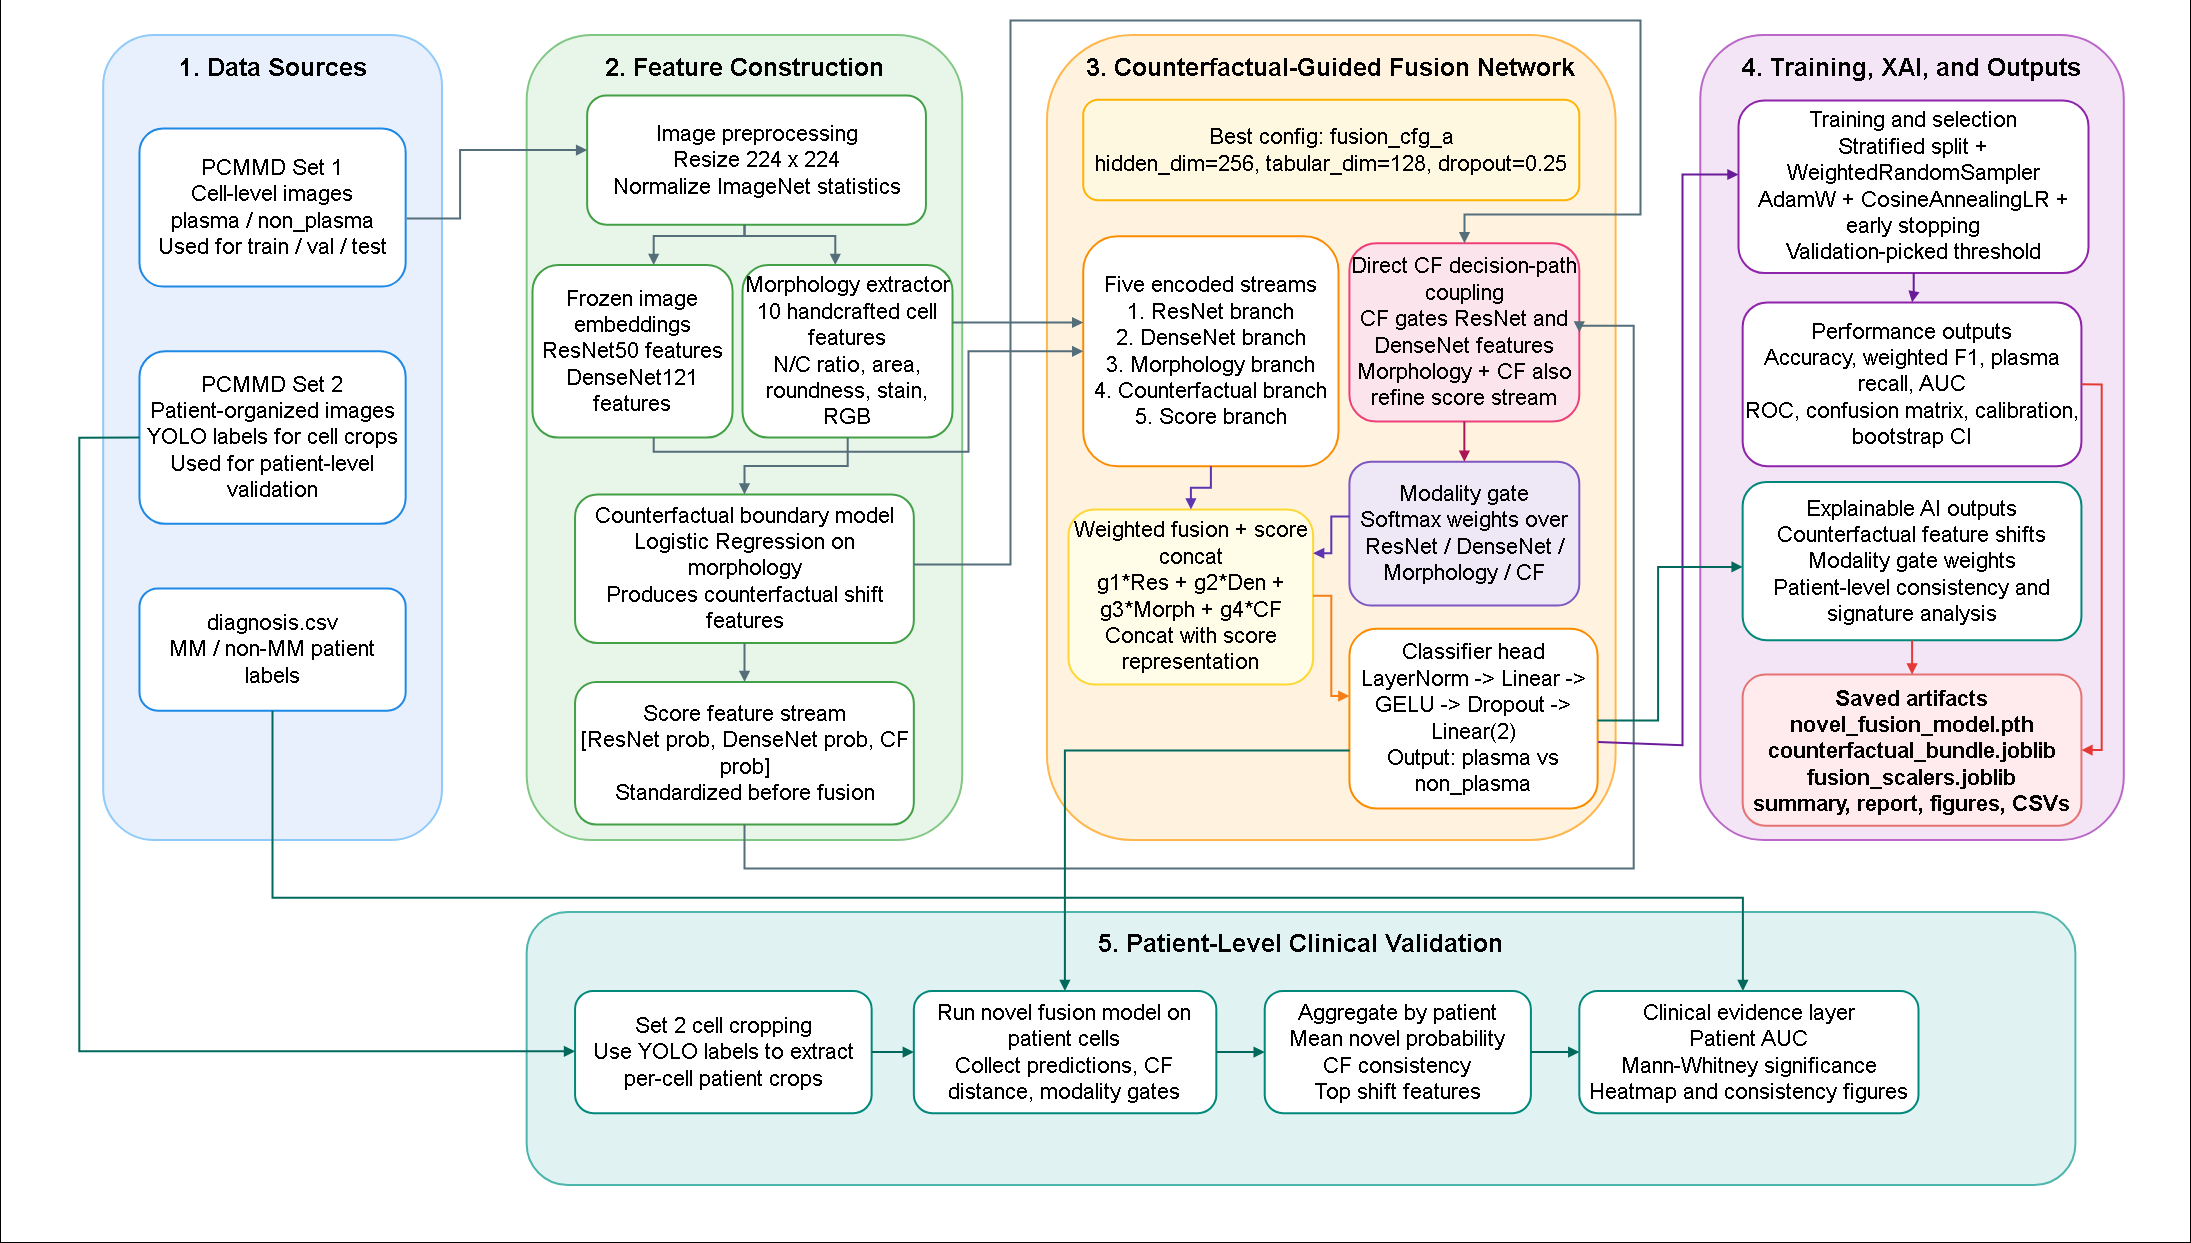
\includegraphics[width=\linewidth]{Architecture_diagram.png}\\[2pt]
\small (b) Detailed fusion architecture.
\end{minipage}
\caption{PlasmaXAI architecture from end-to-end workflow to internal fusion design.}
\label{fig:arch}
\end{figure}
Figure~\ref{fig:arch} shows how image embeddings, morphology descriptors, counterfactual features, and learned gates interact inside the final classifier.

\subsection{Evaluation Protocol}
The deployment operating point is selected on validation data using a precision-recall balanced criterion. Final evaluation reports accuracy, weighted F1, plasma precision, plasma recall, and AUC. Additional analysis includes calibration curves, bootstrap confidence intervals, ablation variants, and patient-level robustness checks based on exact permutation testing and leave-one-patient-out analysis.
\FloatBarrier

\section{Results and Discussion}
\subsection{Core Classification Results}
At the selected operating point, PlasmaXAI achieved 93.42\% accuracy, 93.43\% weighted F1, 91.24\% plasma precision, 94.63\% plasma recall, and 97.76\% AUC. It therefore exceeded the strongest non-PlasmaXAI baselines on the three most deployment-relevant classification criteria: accuracy, precision, and recall. ResNet50 remained the strongest deep baseline by accuracy, while the previous optimized hybrid remained the strongest non-PlasmaXAI precision baseline.

\begin{table}[!htbp]
\centering
\caption{Held-out test performance for the strongest comparison models.}
\label{tab:mainresults}
\begin{tabular}{lccccc}
\toprule
Model & Acc. (\%) & W-F1 (\%) & Prec. (\%) & Recall (\%) & AUC (\%) \\
\midrule
ResNet50 & 91.92 & 91.93 & 89.02 & 93.80 & 97.05 \\
Prev Hybrid & 91.73 & 91.73 & 90.91 & 90.91 & 97.12 \\
DenseNet121 & 89.85 & 89.83 & 90.17 & 87.19 & 96.36 \\
\textbf{PlasmaXAI} & \textbf{93.42} & \textbf{93.43} & \textbf{91.24} & \textbf{94.63} & \textbf{97.76} \\
\bottomrule
\end{tabular}
\end{table}

\begin{figure}[!htbp]
\centering
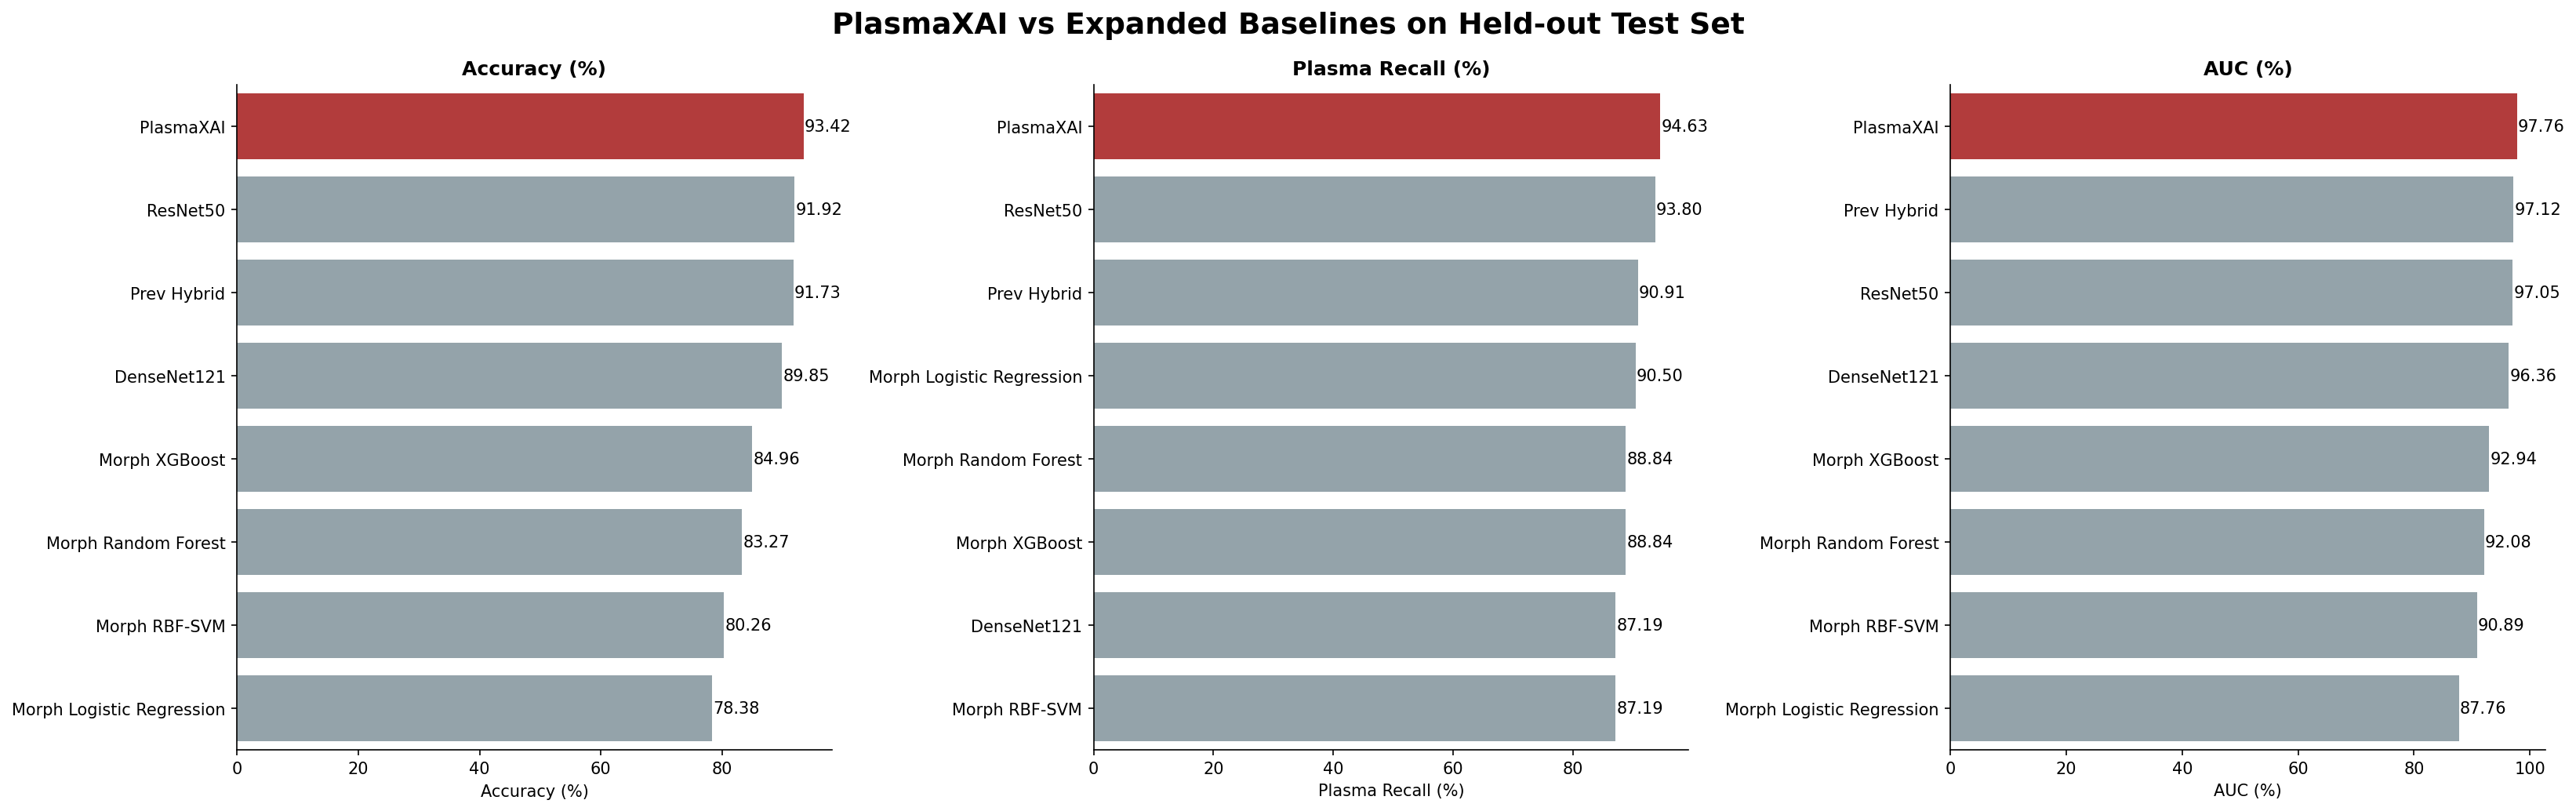
\includegraphics[width=0.90\textwidth]{plasmaxai_model_comparison.png}
\caption{Expanded benchmark comparison showing PlasmaXAI against deep and morphology-based baselines.}
\label{fig:modelcomp}
\end{figure}
Figure~\ref{fig:modelcomp} shows that the full framework maintains the strongest overall balance across the main benchmark metrics.

Bootstrap analysis further indicated that the chosen operating point was stable, with a 95\% confidence interval of 91.16--95.30 for accuracy, 91.30--97.20 for plasma recall, and 96.56--98.63 for AUC. This is important because a clinically useful system must remain strong under resampling rather than depending on a single favorable split.

\subsection{Explainability, Ablation, and Patient-Level Findings}
The explainability pathway is a defining part of PlasmaXAI. Counterfactual analysis shows that the model learns meaningful modality weights while also identifying the dominant morphology shifts that drive its decisions. In practical terms, the classifier produces not only a malignant probability, but also an explanation of which morphologic changes most strongly support that output.

\begin{figure}[!htbp]
\centering
\begin{minipage}[t]{0.48\textwidth}
\centering
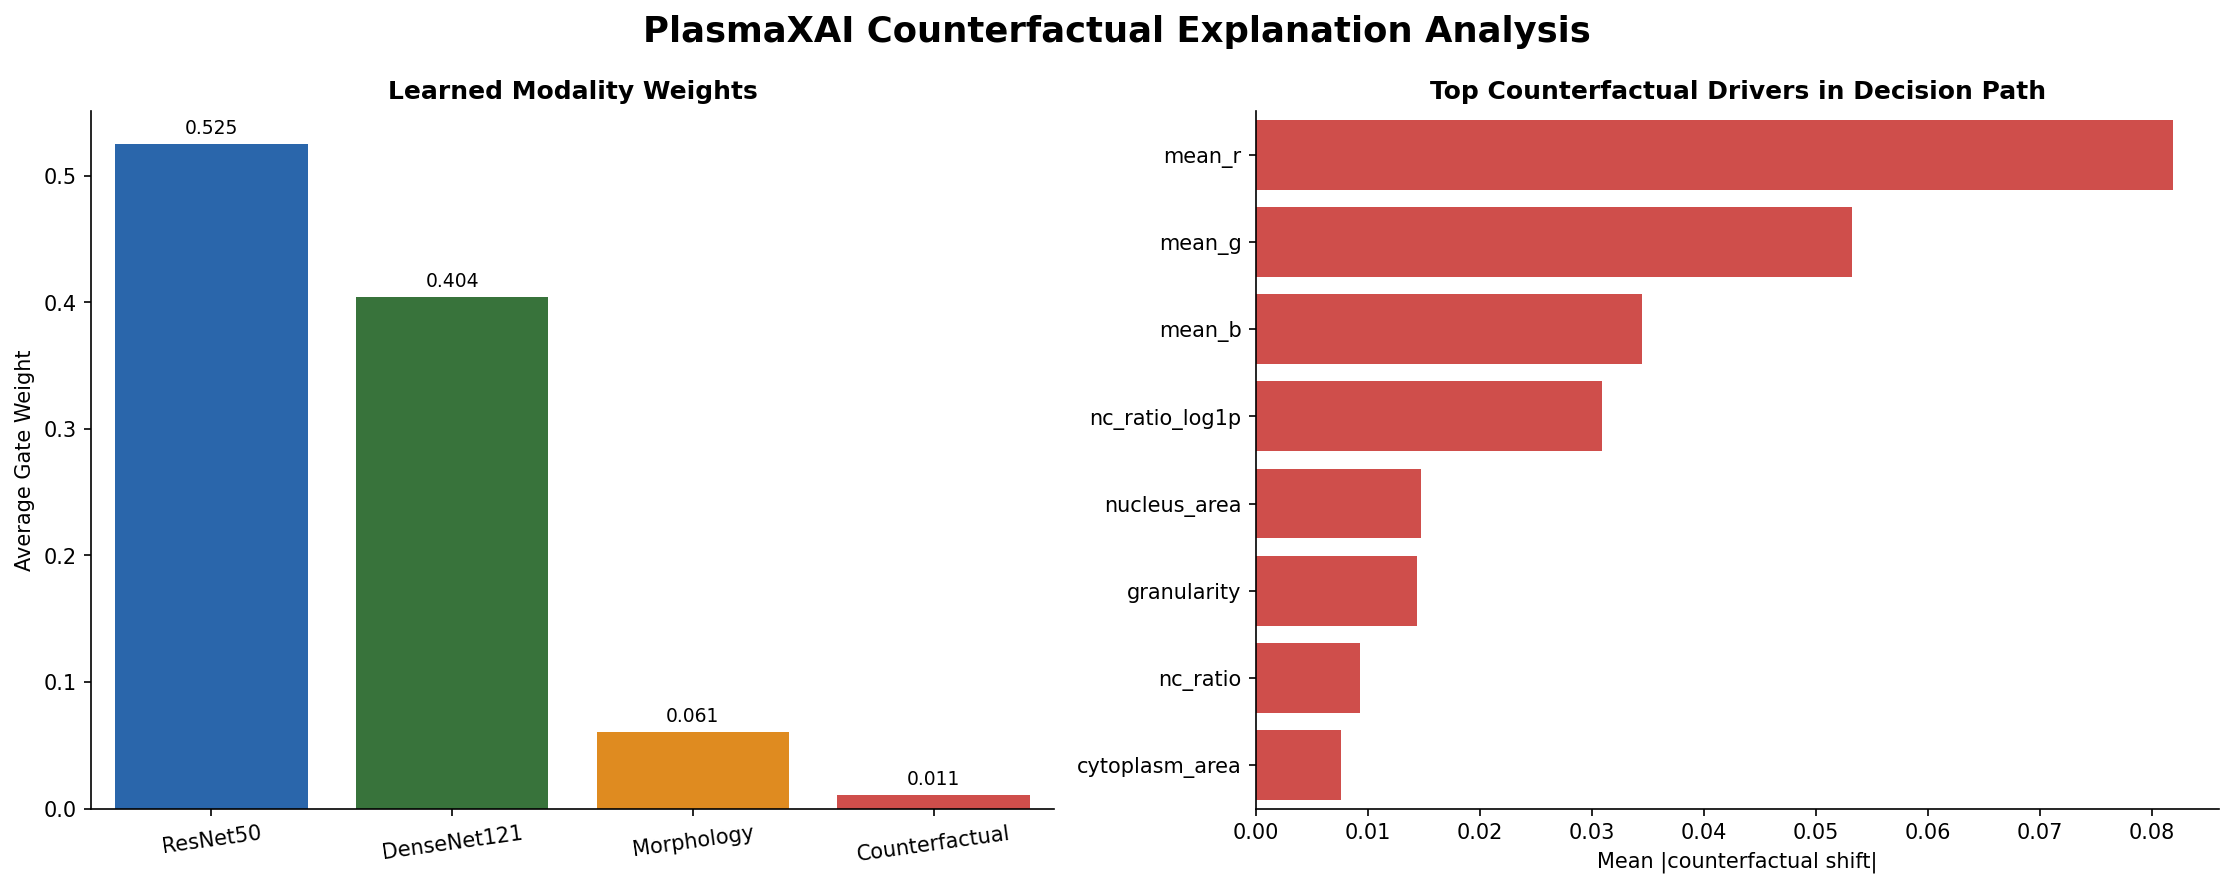
\includegraphics[width=\linewidth]{plasmaxai_counterfactual.png}\\[2pt]
\small (a) Counterfactual explanation analysis.
\end{minipage}\hfill
\begin{minipage}[t]{0.48\textwidth}
\centering
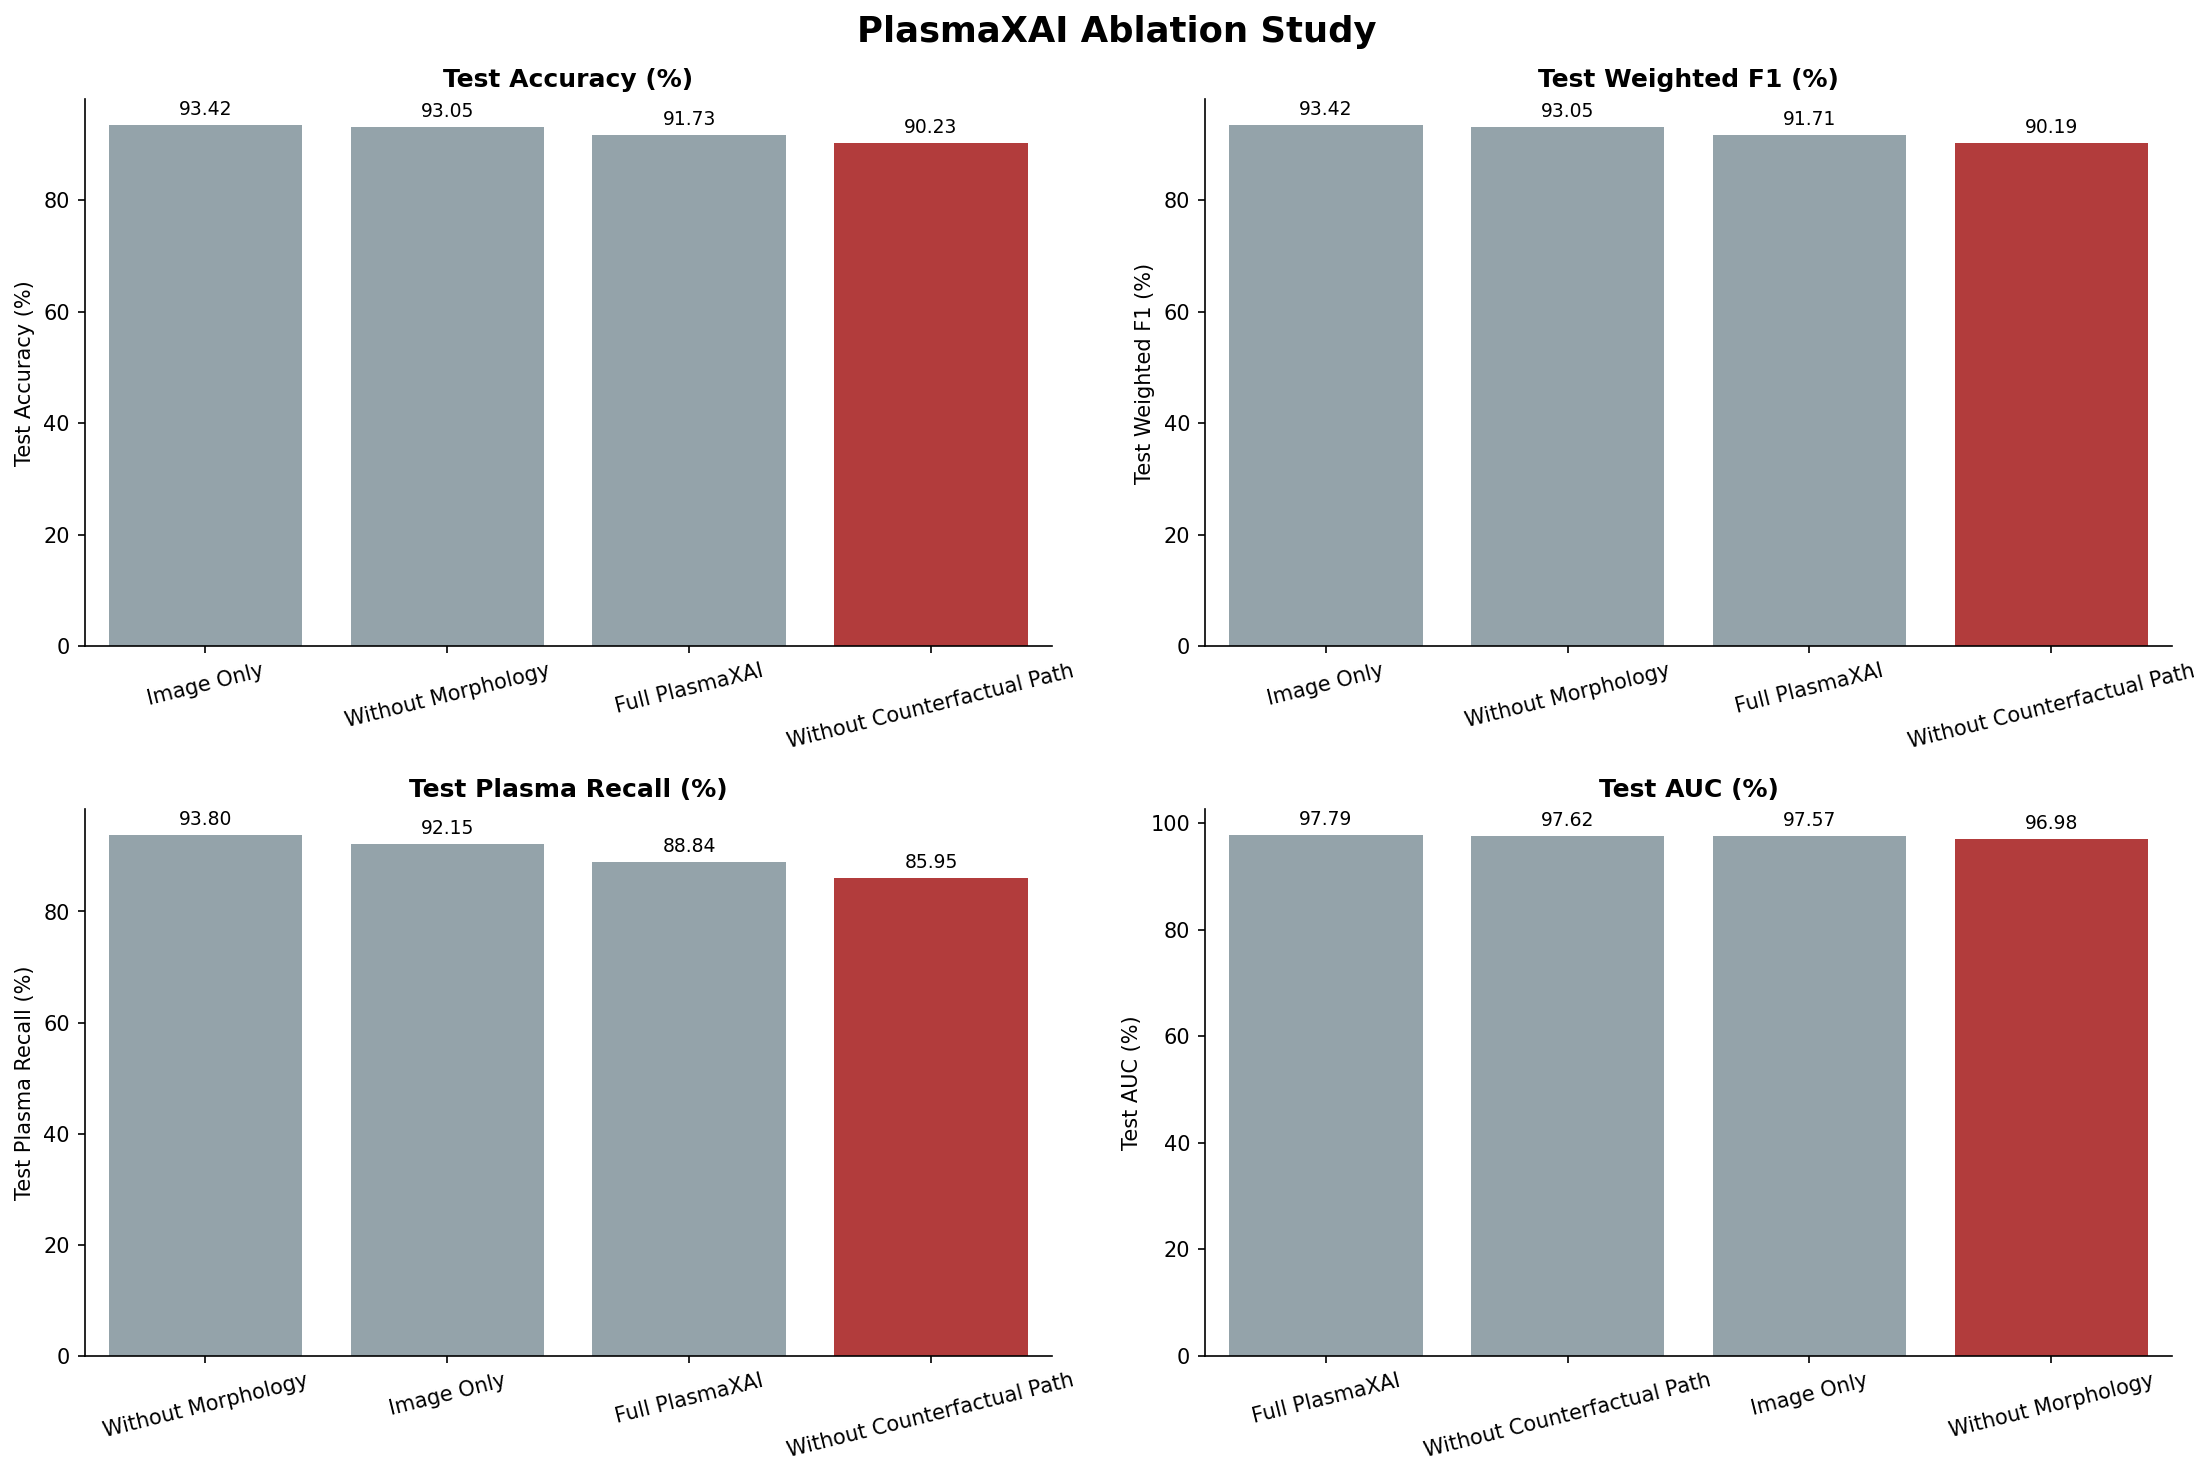
\includegraphics[width=\linewidth]{plasmaxai_ablation.png}\\[2pt]
\small (b) Ablation study overview.
\end{minipage}
\caption{Explainability and ablation evidence for PlasmaXAI.}
\label{fig:xaiablation}
\end{figure}
Figure~\ref{fig:xaiablation} shows that explainability is embedded in the decision path and that removal of the counterfactual branch produces the largest drop in malignant-cell recall.

The ablation study is especially informative. Removing the counterfactual path reduced recall to 85.95\%, substantially below the full system, while the morphology branch also remained useful. This pattern suggests that the main gain in PlasmaXAI comes from the structured interaction between image features and counterfactual morphology reasoning rather than from any single backbone alone.

Patient-level analysis produced an internal AUC of 1.000 on a ten-patient cohort, with exact permutation p-values of 0.0040 one-sided and 0.0079 two-sided. Although encouraging, this should still be interpreted cautiously because the cohort is small and internally sourced. The calibration, robustness, clinical insight, and patient-level signature visualizations therefore serve as supporting analysis rather than definitive clinical proof.

\begin{figure}[!htbp]
\centering
\begin{minipage}[t]{0.48\textwidth}
\centering
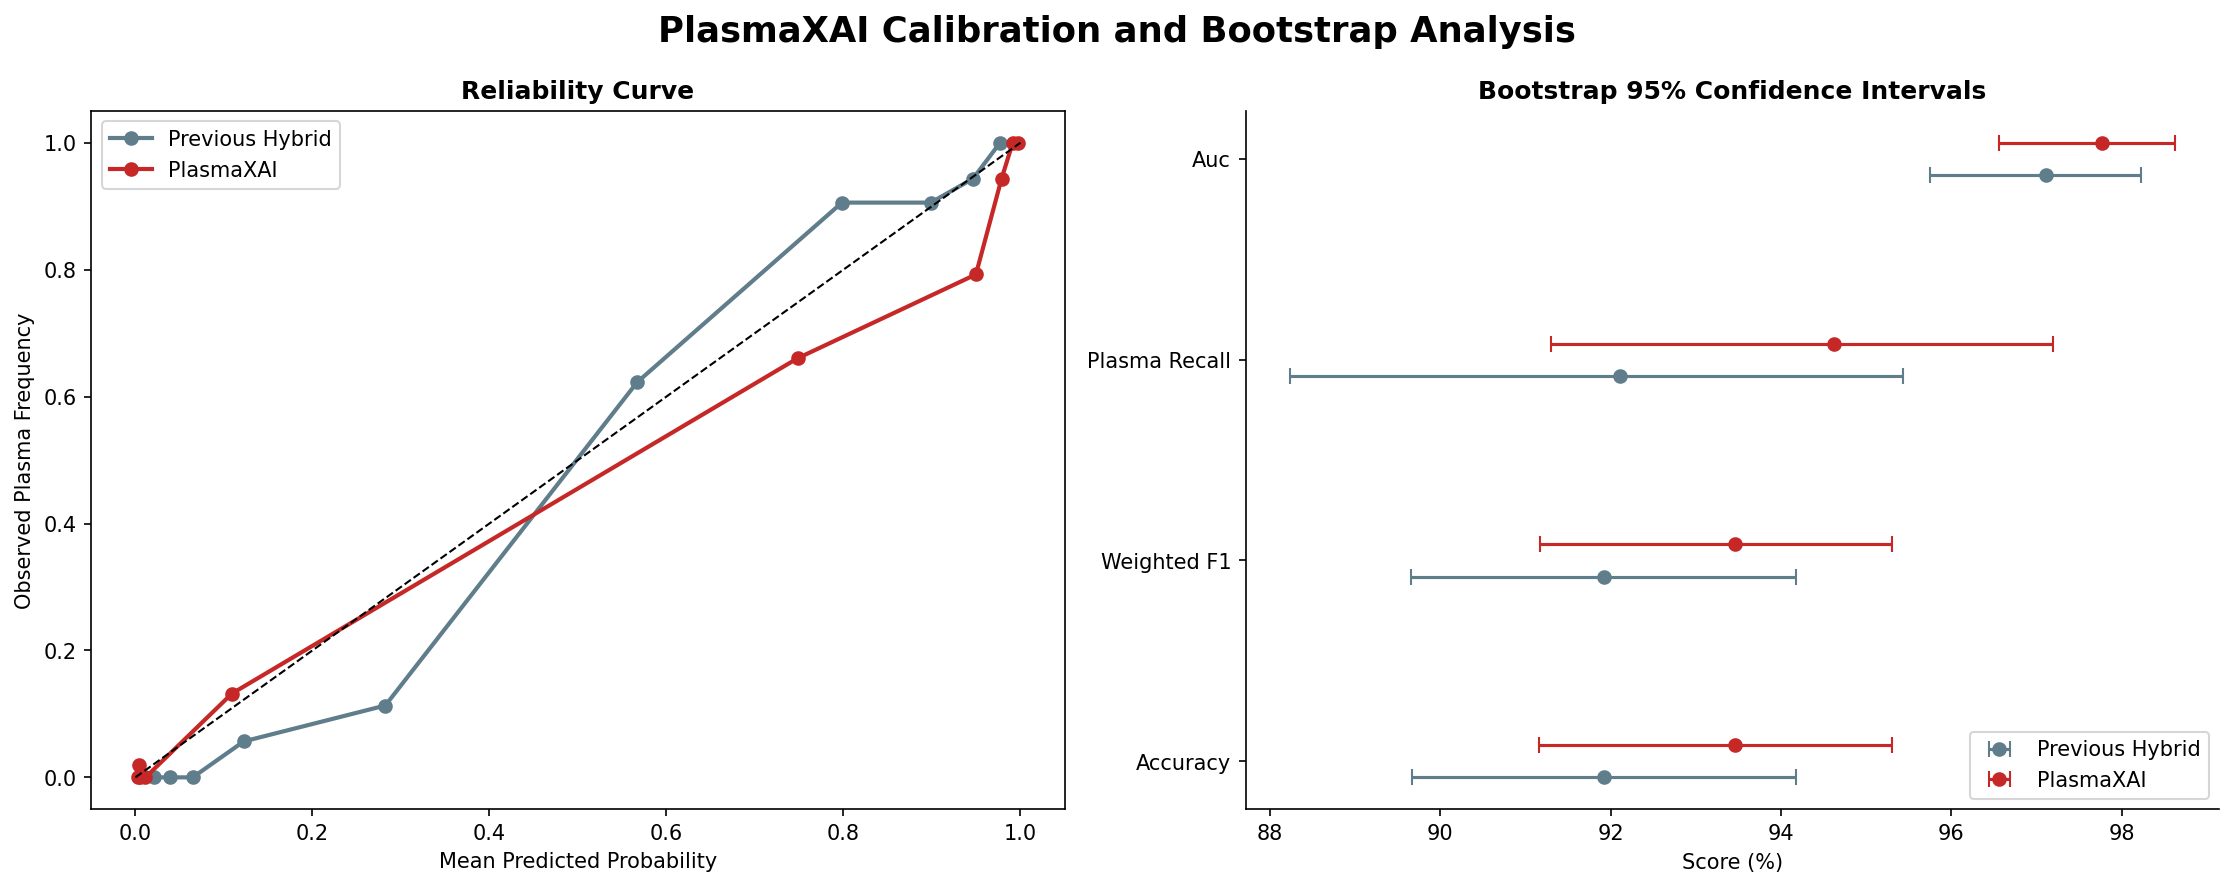
\includegraphics[width=\linewidth]{plasmaxai_calibration_bootstrap.png}\\[2pt]
\small (a) Calibration and bootstrap analysis.
\end{minipage}\hfill
\begin{minipage}[t]{0.48\textwidth}
\centering
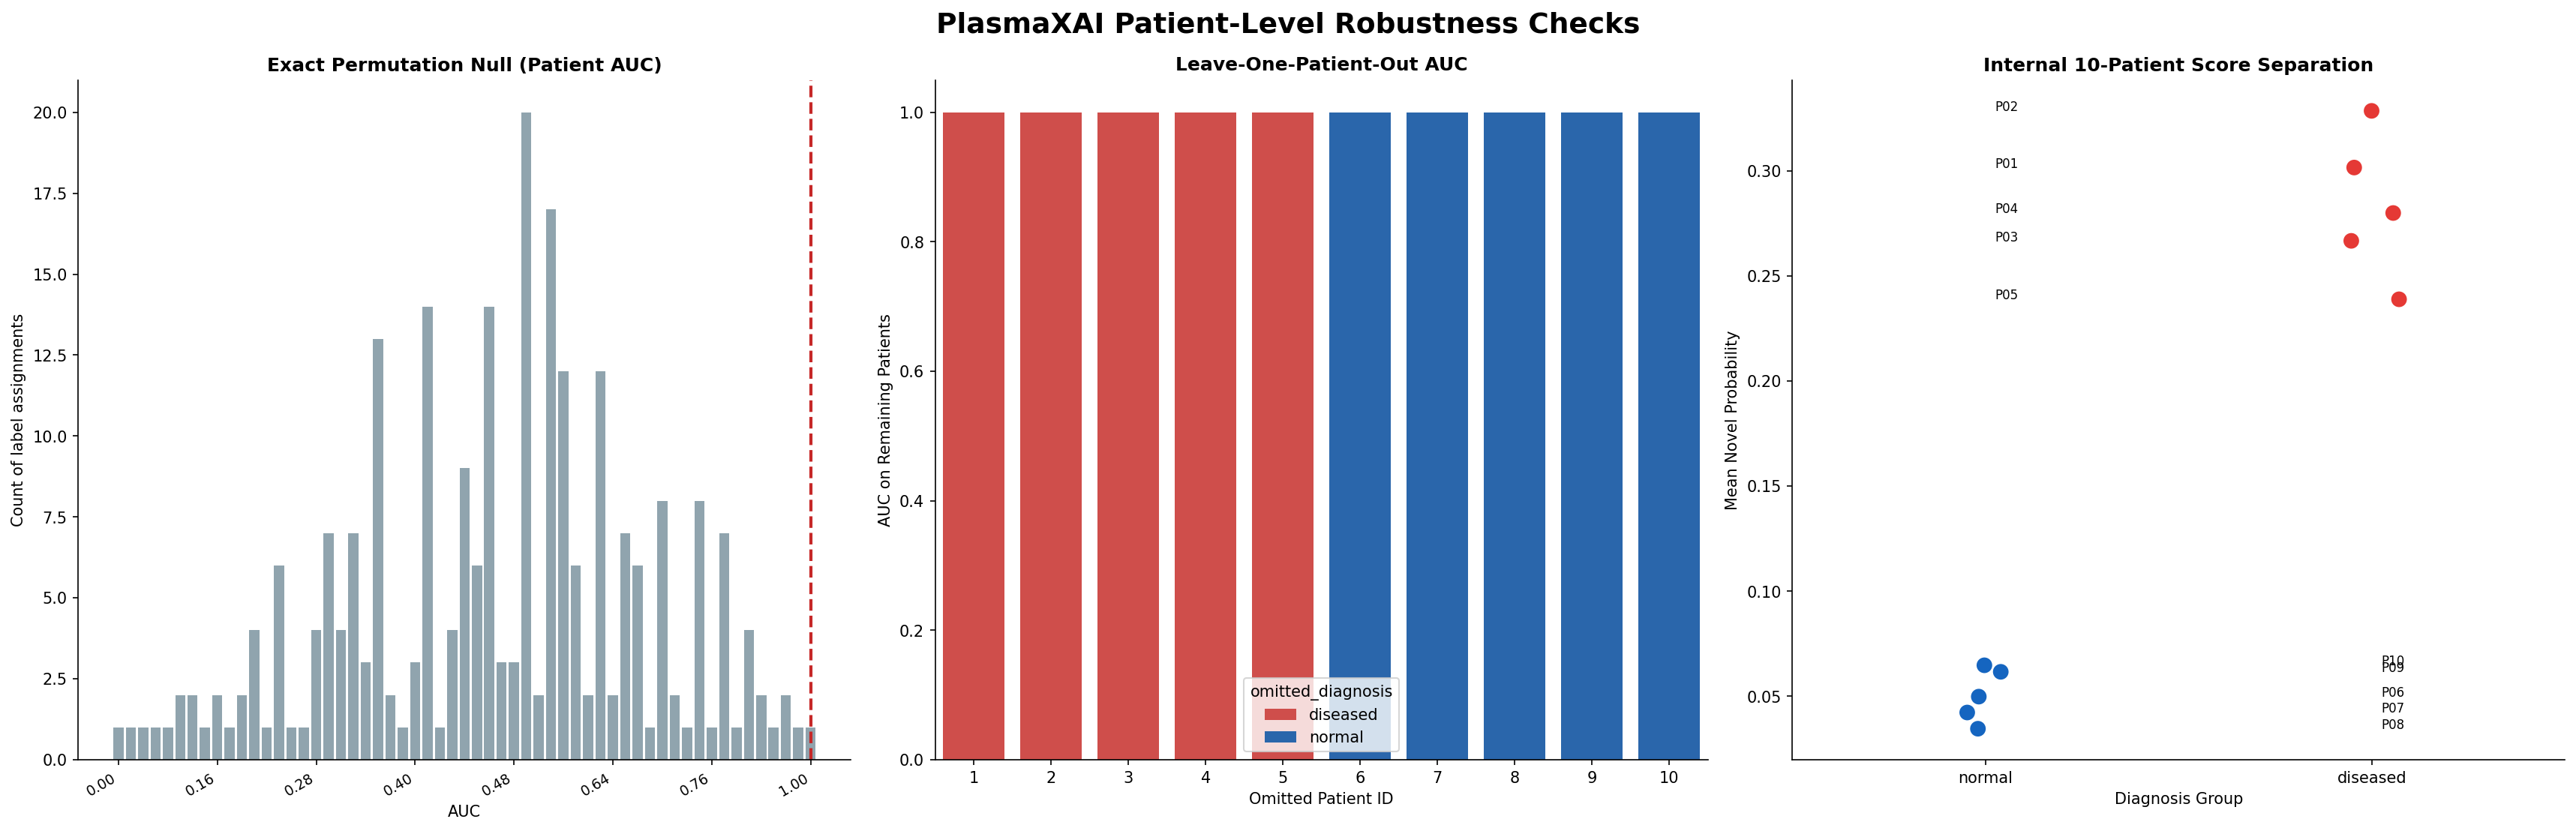
\includegraphics[width=\linewidth]{plasmaxai_patient_robustness.png}\\[2pt]
\small (b) Patient-level robustness checks.
\end{minipage}
\caption{Reliability analysis for PlasmaXAI at the selected operating point.}
\label{fig:reliability}
\end{figure}
Figure~\ref{fig:reliability} shows that the final operating point is stable under resampling, but also reminds us that internal patient separation is not a substitute for external validation.

\begin{figure}[!htbp]
\centering
\begin{minipage}[t]{0.48\textwidth}
\centering
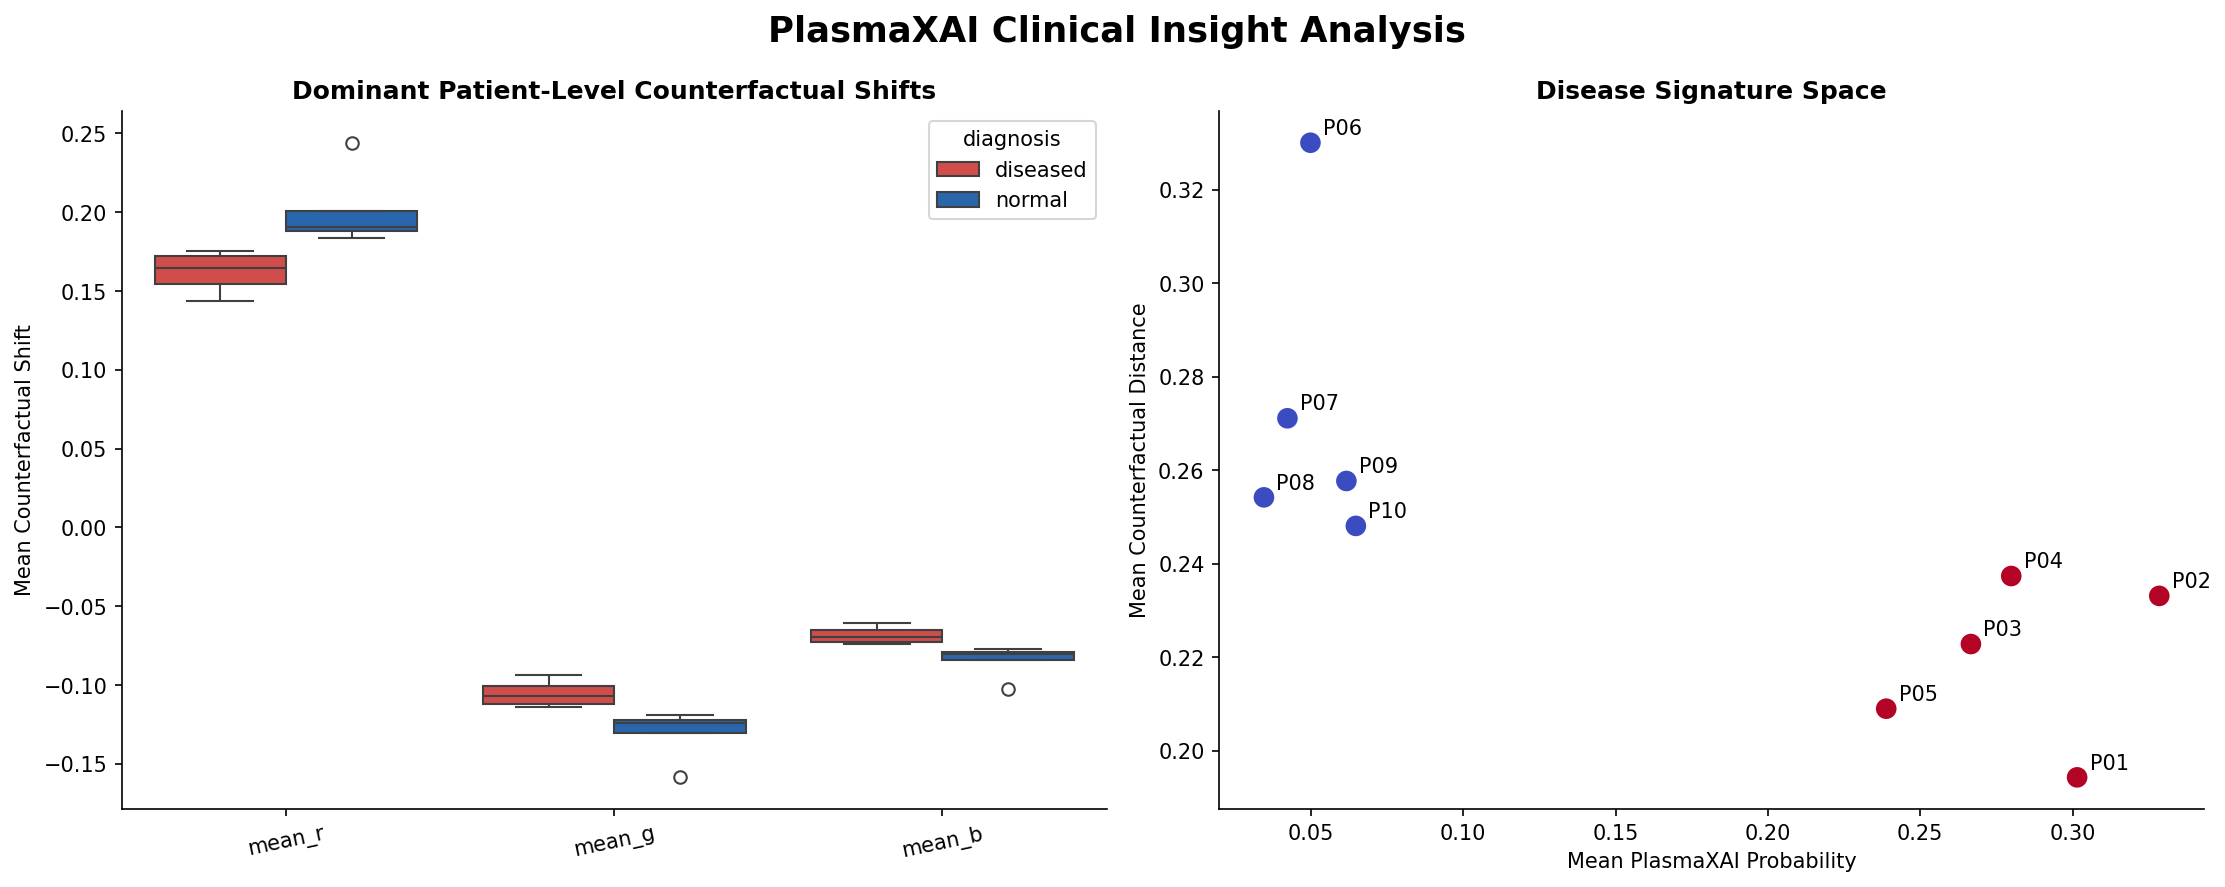
\includegraphics[width=\linewidth]{plasmaxai_clinical_insight.png}\\[2pt]
\small (a) Clinical insight analysis.
\end{minipage}\hfill
\begin{minipage}[t]{0.48\textwidth}
\centering
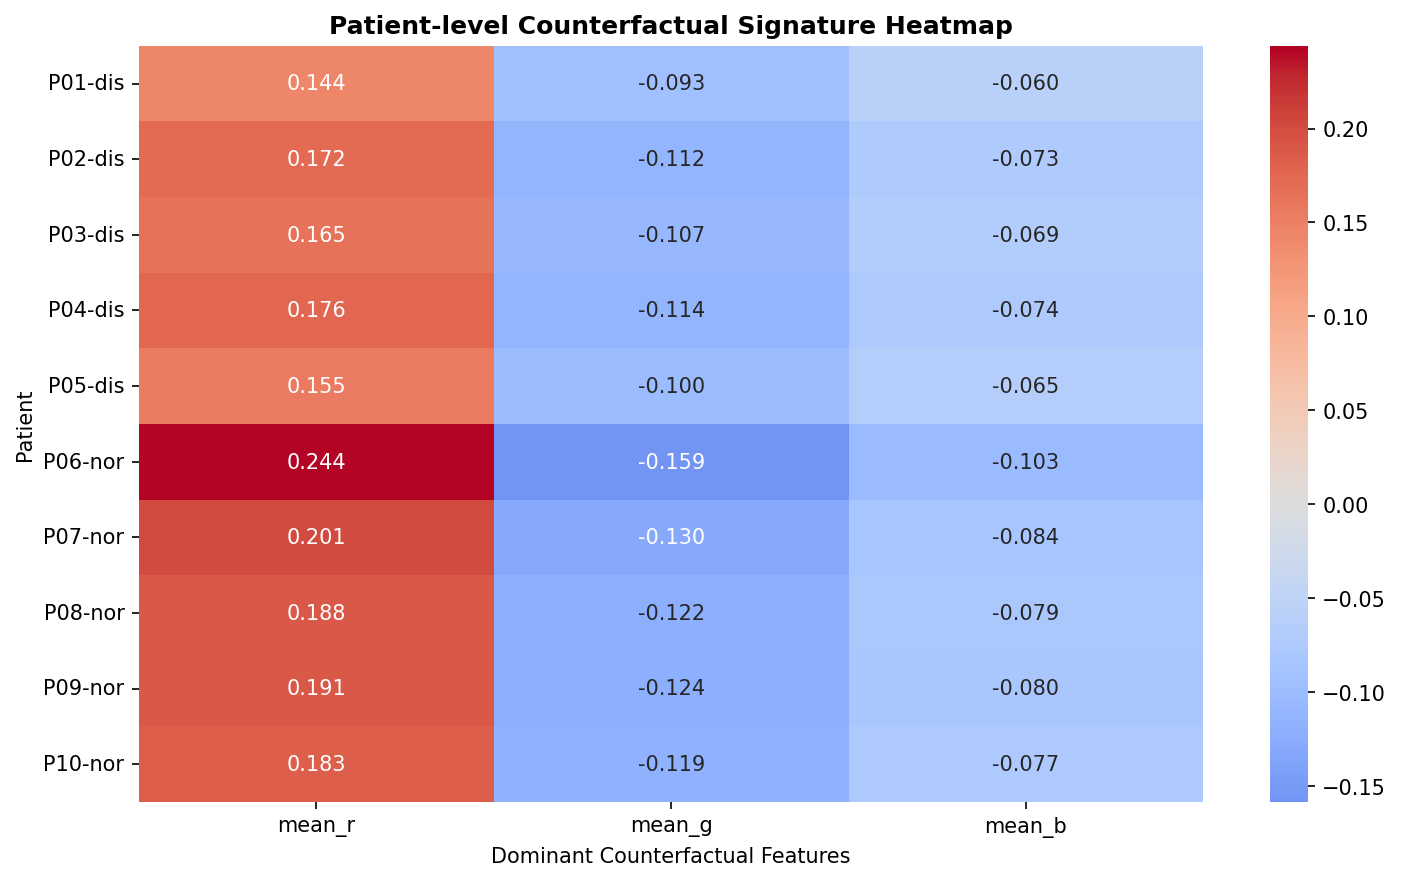
\includegraphics[width=\linewidth]{plasmaxai_patient_heatmap.png}\\[2pt]
\small (b) Patient-level heatmap.
\end{minipage}
\caption{Patient-level clinical interpretation produced by PlasmaXAI.}
\label{fig:clinicalpanel}
\end{figure}
Figure~\ref{fig:clinicalpanel} summarizes the disease-signature space and the patient-wise counterfactual morphology pattern learned by the framework.

Taken together, the results position PlasmaXAI as a strong explainable classifier for plasma cell recognition. Its practical value lies not only in improved classification, but also in the fact that model behavior can be interrogated through counterfactual features, uncertainty summaries, and patient-level consistency analysis.
\FloatBarrier

\section{Conclusion}
This paper presents PlasmaXAI as an explainable fusion framework for malignant plasma cell recognition. The model integrates deep image embeddings, morphology descriptors, and counterfactual reasoning into a unified decision path and achieves strong held-out performance while preserving interpretability. PlasmaXAI outperforms key baselines, shows meaningful sensitivity to removal of the counterfactual branch, and provides transparent diagnostic figures that support auditing and clinician-in-the-loop validation. The major limitation is the lack of external patient-level validation. Future work should therefore focus on broader hematopathology cohorts, stain-robust generalization, and prospective clinical evaluation.

\begin{thebibliography}{99}
\bibitem{mmreview} Rajkumar, S.V.: Multiple myeloma: 2022 update on diagnosis, risk-stratification, and management. Am. J. Hematol. 97, 1086--1107 (2022)
\bibitem{litjens} Litjens, G., Kooi, T., Bejnordi, B.E., et al.: A survey on deep learning in medical image analysis. Med. Image Anal. 42, 60--88 (2017)
\bibitem{bera} Bera, K., Schalper, K.A., Rimm, D.L., Velcheti, V., Madabhushi, A.: Artificial intelligence in digital pathology---new tools for diagnosis and precision oncology. Nat. Rev. Clin. Oncol. 16, 703--715 (2019)
\bibitem{resnet} He, K., Zhang, X., Ren, S., Sun, J.: Deep residual learning for image recognition. In: Proceedings of the IEEE Conference on Computer Vision and Pattern Recognition, pp. 770--778 (2016)
\bibitem{densenet} Huang, G., Liu, Z., van der Maaten, L., Weinberger, K.Q.: Densely connected convolutional networks. In: Proceedings of the IEEE Conference on Computer Vision and Pattern Recognition, pp. 4700--4708 (2017)
\bibitem{wachter} Wachter, S., Mittelstadt, B., Russell, C.: Counterfactual explanations without opening the black box: Automated decisions and the GDPR. Harv. J. Law Technol. 31(2), 841--887 (2018)
\bibitem{diceml} Mothilal, R.K., Sharma, A., Tan, C.: Explaining machine learning classifiers through diverse counterfactual explanations. In: FAT* 2020, pp. 607--617 (2020)
\bibitem{calibration} Guo, C., Pleiss, G., Sun, Y., Weinberger, K.Q.: On calibration of modern neural networks. In: Proceedings of the 34th International Conference on Machine Learning, pp. 1321--1330 (2017)
\bibitem{unet} Ronneberger, O., Fischer, P., Brox, T.: U-Net: Convolutional networks for biomedical image segmentation. In: MICCAI 2015. LNCS, vol. 9351, pp. 234--241. Springer, Cham (2015)
\bibitem{attentionunet} Oktay, O., Schlemper, J., Folgoc, L.L., et al.: Attention U-Net: Learning where to look for the pancreas. arXiv preprint arXiv:1804.03999 (2018)
\bibitem{janowczyk} Janowczyk, A., Madabhushi, A.: Deep learning for digital pathology image analysis: A comprehensive tutorial with selected use cases. J. Pathol. Inform. 7, 29 (2016)
\bibitem{campanella} Campanella, G., Hanna, M.G., Geneslaw, L., et al.: Clinical-grade computational pathology using weakly supervised deep learning on whole slide images. Nat. Med. 25, 1301--1309 (2019)
\bibitem{lime} Ribeiro, M.T., Singh, S., Guestrin, C.: "Why should I trust you?": Explaining the predictions of any classifier. In: Proceedings of the 22nd ACM SIGKDD International Conference on Knowledge Discovery and Data Mining, pp. 1135--1144 (2016)
\bibitem{gradcam} Selvaraju, R.R., Cogswell, M., Das, A., et al.: Grad-CAM: Visual explanations from deep networks via gradient-based localization. In: Proceedings of the IEEE International Conference on Computer Vision, pp. 618--626 (2017)
\bibitem{shap} Lundberg, S.M., Lee, S.-I.: A unified approach to interpreting model predictions. In: Advances in Neural Information Processing Systems, pp. 4765--4774 (2017)
\end{thebibliography}

\end{document}
